%%%%%%%%%%%%%%%%%%%%%%%%%%%%%%%%%%%%%%%%%%%%%%%%%%%%%%%%%%%%%%%%%%%%%%%%%%
%%%%%                         CHAPITRE 3                            %%%%%%
%%%%%%%%%%%%%%%%%%%%%%%%%%%%%%%%%%%%%%%%%%%%%%%%%%%%%%%%%%%%%%%%%%%%%%%%%%

\lhead[\fancyplain{}{\leftmark}]%Pour les pages paires \bfseries
      {\fancyplain{}{}} %Pour les pages impaires
\chead[\fancyplain{}{}]%
      {\fancyplain{}{}}
\rhead[\fancyplain{}{}]%Pour les pages paires 
      {\fancyplain{}{\rightmark}}%Pour les pages impaires \bfseries
\lfoot[\fancyplain{}{}]%
      {\fancyplain{}{}}
\cfoot[\fancyplain{}{\thepage}]%\bfseries
      {\fancyplain{}{\thepage}} %\bfseries
\rfoot[\fancyplain{}{}]%
     {\fancyplain{}{\scriptsize}}


%%%%%%%%%%%%%%%%%%%%%%%%%%%%%%%%%%%%%%%%%%%%%%%%%%%%%%%%%%%%%%%%%%%%%%%%%%
%%%%%                      Start part here                          %%%%%%
%%%%%%%%%%%%%%%%%%%%%%%%%%%%%%%%%%%%%%%%%%%%%%%%%%%%%%%%%%%%%%%%%%%%%%%%%%

\chapter{Proposed solution: Pose2Sim Python package}
\label{ch:3}

%==============================================================================	Résumé du chapitre

\begin{center}
\rule{0.7\linewidth}{.5pt}
\begin{minipage}{0.7\linewidth}
\smallskip

\textit{This chapter present our proposed solution, the Pose2Sim python package. This package is meant to consitute a user-friendly bridge between the most common 2D pose detection algorithms, and the OpenSim software so as to provide physically consistent 3D kinematics. Code is available at \url{https://github.com/perfanalytics/pose2sim} \newline \newline
This chapter is adapted from the article published in the Journal of Open Source Software "Pose2Sim: An Open-source Python Package for multiview markerless kinematics" \cite{Pagnon2022b}}

%\smallskip
\end{minipage}
\smallskip
\rule{0.7\linewidth}{.5pt}
\end{center}

\minitoc
\newpage


\section{Introduction to the workflow}
Pose2Sim provides a framework for 3D markerless kinematics, as an alternative to the more usual marker-based motion capture methods. Pose2Sim stands for "OpenPose to OpenSim", as it connects two of the most widely recognized (and open-source) pieces of software in their respective fields: OpenPose \cite{Cao2019}, a 2D human pose estimation neural network; and OpenSim \cite{Delp2007,Seth2018}, a 3D biomechanics analysis software. Pose2Sim is accessible at \url{https://github.com/perfanalytics/pose2sim}.

The repository presents a framework which consists in (Figures~\ref{fig_pipeline}):
\begin{enumerate}[itemsep=-0.5em, topsep=0pt, leftmargin=*]
      \item Preliminary 2D joint coordinate detections from multiple videos, e.g. with OpenPose.
      \item Pose2Sim core, including 4 customizable steps:
      \begin{enumerate}[before=\vspace{-0.5\baselineskip}, nosep]
            \item Camera calibration.
            \item 2D tracking of the person of interest.
            \item 3D keypoint triangulation, and storage in a .trc file.
            \item 3D coordinate filtering.
      \end{enumerate}
      \item Scaling to each individual subject, and inverse kinematics via OpenSim, and storage of the full-body 3D joint angles.
\end{enumerate}

\begin{figure}[hbtp]
	\centering
	\def\svgwidth{1\columnwidth}
	\fontsize{10pt}{10pt}\selectfont
	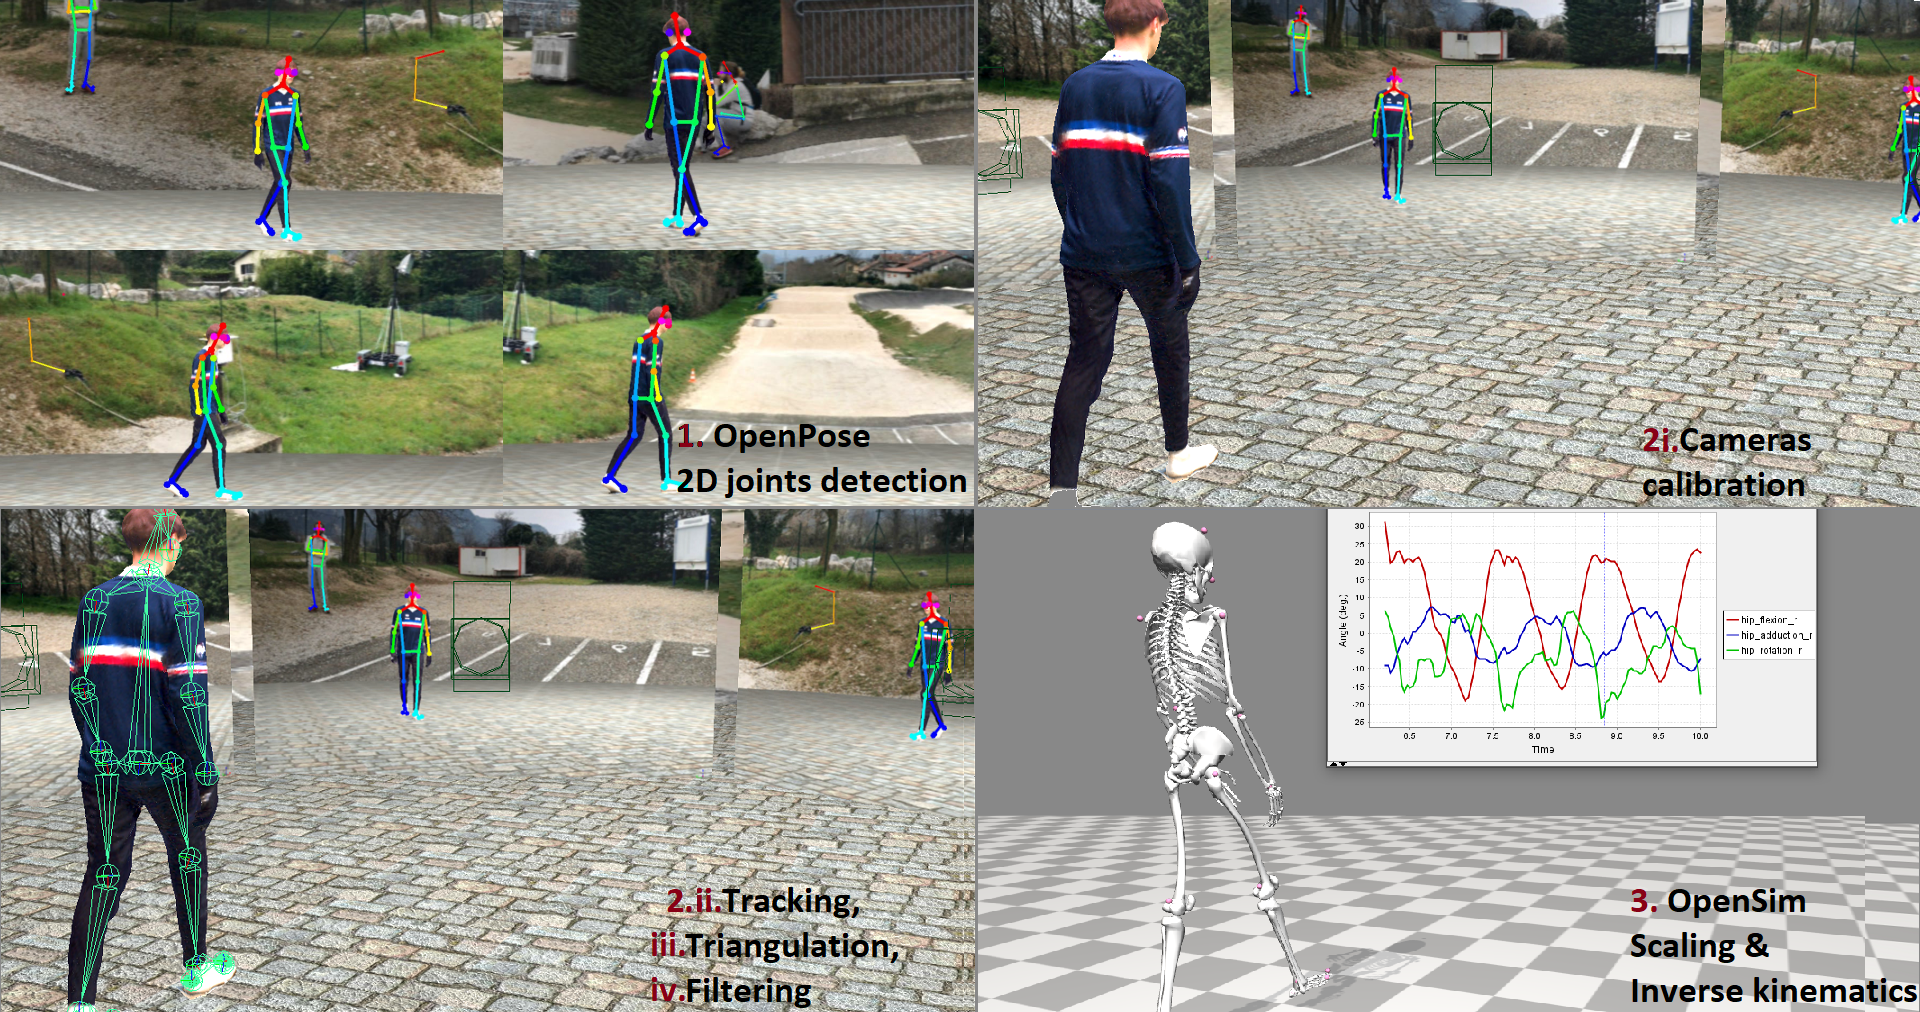
\includegraphics[width=\linewidth]{"../Chap3/Figures/Pipeline.png"}
	\caption{Pose2Sim pipeline: (1) 2D joints detection; (2i) camera calibration; (2ii–iv) tracking the person of interest, triangulating their coordinates, and filtering them; (3) scaling the subject, and constraining their 3D coordinates to a physically consistent OpenSim skeletal model}
	\label{fig_pipeline}
\end{figure}
\FloatBarrier

Each task is easily customizable, and requires only moderate Python skills. The whole workflow runs from any video cameras, on any computer, equipped with any operating system (although OpenSim has to be compiled from source on Linux.) Pose2Sim has already been used and tested in a number of situations (walking, running, cycling, dancing, balancing, swimming, boxing), and published in peer-reviewed scientific publications assessing its robustness (see Chapter 4 on \nameref{ch:4}) \cite{Pagnon2021} and its accuracy (see Chapter 5 on \nameref{ch:5}) \cite{Pagnon2022}. Its results for inverse kinematics were deemed good when compared to marker-based ones, with errors generally below 4.0° across several activities, on both lower and on upper limbs. The combination of its ease of use, customizable parameters, and high robustness and accuracy makes it promising, especially for "in-the-wild" sports movement analysis.


\section{2D pose detection}

% OpenPose, for example, is a widespread open-source software which provides 2D joint coordinate estimates from videos. These coordinates can then be triangulated in order to produce 3D positions. 


\section{Pose2Sim core}
\subsection{Tracking of the person viewed by the most cameras}
\blindtext

\subsection{Triangulating by weighted direct linear transform}

% Open source tools for triangulating
% Some tools have been released open source
% Aside from ours (see Chapter 3 on \nameref{ch:3}), a number a tools have been made available for such triangulation: the experimental OpenPose 3D reconstruction module [Hidalgo2021], the FreeMoCap Python and Blender toolbox [Matthis2022], or the pose3d Matlab toolbox [Sheshadri2020]. Yet, when it comes to the biomechanical analysis of human motion, it is often more useful to obtain joint angles than joint center positions in space. Joint angles allow for better comparison among trials and individuals, and they represent the first step for other analyses such as inverse dynamics. EasyMocap ?


\subsection{Filtering}
\blindtext


\section{Pose2Sim skeletal model}

A full-body OpenSim \cite{Delp2007,Seth2018} skeletal model with OpenPose keypoints is provided, as well as scaling and inverse kinematics setup files.

OpenSim is another widespread open-source software which helps compute 3D joint angles, usually from marker coordinates. It lets scientists define a detailed musculoskeletal model, scale it to individual subjects, and perform inverse kinematics with customizable biomechanical constraints. It provides other features such as net calculation of joint moments or resolution of individual muscle forces, although this is beyond the scope of our contribution.


\section{Limitations and perspectives}
\blindtext


\section{Helper functions and vizualisation tools}
\blindtext



\section{Exemples}

\FloatBarrier
\subsection{Tableaux}

Générateur en ligne \href{http://www.tablesgenerator.com/latex_tables}{ici}. \\

Un exemple de tableau générée par cet outil est présenté Table~\ref{tableau_exemple}.

\begin{table}[]
\centering
\begin{tabular}{c|c|c|c|}
\cline{2-4}
                               & \textbf{A}                 & \textbf{B} & \textbf{C} \\ \hline
\multicolumn{1}{|c|}{$\alpha$} & \multicolumn{3}{c|}{\textit{fusion}}                 \\ \hline
\multicolumn{1}{|c|}{$\beta$}  & \multirow{2}{*}{\textit{}} & \textit{1} & \textit{2} \\ \cline{1-1} \cline{3-4} 
\multicolumn{1}{|c|}{$\Delta$} &                            & \textit{3} & \textit{4} \\ \hline
\end{tabular}
\caption{Exemple de tableau}
\label{tableau_exemple}
\end{table}
